\documentclass[a4paper, 12pt, notitlepage]{article}
\usepackage[brazil]{babel}
\usepackage[utf8]{inputenc}
\usepackage[backend=biber]{biblatex}
\usepackage[hmargin=2cm,vmargin=3cm,bmargin=3cm]{geometry}
\usepackage{enumerate}
\usepackage{graphicx}
\usepackage{float}
\usepackage{mathtools}
\usepackage{physics}
\usepackage{amsmath,amssymb,amsthm}  %pacotes para matemática, opções de indentação, e links
\usepackage{caption}  % caption to minipages
\usepackage{indentfirst}
\usepackage{makeidx}
\usepackage{hyperref}
\hypersetup{colorlinks=false}
\usepackage[T1]{fontenc}
\usepackage{microtype}

\usepackage[sc,osf]{mathpazo}   % With old-style figures and real smallcaps.
\linespread{1.030}              % Palatino leads a little more leading

% Euler for math and numbers
\usepackage[euler-digits,small]{eulervm}
\AtBeginDocument{\renewcommand{\hbar}{\hslash}}

% Latex plots and drawings
\usepackage{tikz}
\usetikzlibrary{arrows.meta, angles, quotes}
\tikzset{>={Latex[width=3mm,length=3mm]}}  %setas mais visíveis no tikz
\usepackage{pgfplots}
\usepgfplotslibrary{fillbetween}

% some useful math shortcuts
\newtheorem{lema}{Lema }
\newtheorem{teorema}{Teorema }
\newtheorem{corolario}[teorema]{Corolário }
\newtheorem{definicao}{Definição }[section]
\newtheorem{postulado}{Postulado }[section]
\newtheorem{proposicao}{Proposição }[section]
\newtheorem{problema}{Problema }
\newcommand{\cart}{\times}
\newcommand{\ses}{\Longleftrightarrow}
\newcommand{\entao}{\Longrightarrow}
\newcommand{\e}{\wedge}
\newcommand{\ou}{\vee}
\newcommand{\vazio}{\varnothing}
\newcommand{\sobre}{\longrightarrow}
\newcommand{\N}{\mathbb{N}}
\newcommand{\Q}{\mathbb{Q}}
\newcommand{\R}{\mathbb{R}}
\newcommand{\Z}{\mathbb{Z}}
\newcommand{\La}{\mathcal{L}}
\newcommand{\cmod}[3]{#1 \equiv #2\textrm{ (mod }#3\textrm{)}}
\newcommand{\tq}{\textrm{ tal que }}
\renewcommand{\qedsymbol}{$\blacksquare$}
\newcommand{\dsum}{\displaystyle \sum}
\newcommand{\divg}[1]{\vec{\nabla} \cdot #1}
\newcommand{\rot}[1]{\vec{\nabla} \times #1}
\newcommand{\vecb}[1]{\mathbf{ #1}}
\newcommand{\veb}[1]{\mathbf{\hat{#1}}}

\bibliography{townsend}

\begin{document}
\title{Resolução da Prova 3 de Mecânica Quântica I\\ (F689, Turma B, 1o. semestre de 2015)}
\author{Pedro Rangel Caetano\footnote{Email: p.r.caetano@gmail.com}} 
\date{Universidade Estadual de Campinas, 1o. semestre de 2017}
\maketitle

%\tableofcontents
%\pagebreak

\begin{enumerate}

% Problema 1
\addcontentsline{toc}{section}{Problema 1}
\item Confira problema 12 da lista 3.

% Problema 2
\addcontentsline{toc}{section}{Problema 2}
\item Um sistema esta no estado

\[
  \psi(t = 0) = \frac{1}{2} \left(\frac{3}{2\pi}\right)^{1/2} \sin \theta e^{-i\phi}  
\]

\begin{enumerate}[(A)]
  \item Em qual estado de momento angular total e momento angular na direção z o sistema está?
  
  \textbf{Resolução: }
  
  No formulário foi fornecido que
  
  \[
  Y^1_1 = -\frac{1}{2}\left(\frac{3}{2\pi}\right)^{1/2}\sin \theta e^{i\phi}
  \]
  
  \noindent e que
  
  \[
  Y_l^{-m} = (-1)^m(Y^m_l)^{\ast}
  \]
  
  \noindent portanto  
  
  \[
  Y^{-1}_1 = \frac{1}{2}\left(\frac{3}{2\pi}\right)^{1/2}\sin \theta e^{-i\phi}
  \]
  
  \noindent e $\psi(t = 0) = Y^{-1}_1$. Denotando por $\ket{\psi(t=0)}$ o ket correpondente à função de onda $\psi(t=0)$ temos então
  
  \[
  \ket{\psi(t=0)} = \ket{l=1,\,m=-1}
  \]
  
  O sistema está no autoestado de $L^2$ com autovalor $2\hbar^2$ e de $L_z$ com autovalor $-\hbar$.
  
  \item Se fossemos medir o momento angular na direção x, $\hat{L}_x$, quais são os valores possível que poderíamos achar? Justifique.
  
  \textbf{Resolução:}
  
  Quando $l=1$, o formulário fornece que a representação de $L_x$ na base z é
  
  \[
  L_x = \frac{\hbar}{\sqrt{2}}\begin{pmatrix}
  0 & 1 & 0 \\
  1 & 0 & 1 \\
  0 & 1 & 0
  \end{pmatrix}
  \]
  
  Os valores possíveis são os autovalores desta matriz:
  
  \begin{align*}
  \begin{vmatrix}
  -\lambda & \hbar/\sqrt{2} & 0 \\
  \hbar/\sqrt{2} & -\lambda & \hbar/\sqrt{2} \\
  0 & \hbar/\sqrt{2} & -\lambda
  \end{vmatrix} &= 0 \\
  -\lambda^3 + 2\lambda \frac{\hbar^2}{2} &= 0 \\
  \lambda\left(\hbar - \lambda\right)\left(\hbar + \lambda\right) &= 0
  \end{align*}
  
  De onde é claro que os valores possíveis são $-\hbar$, $0$ e $\hbar$.
  
  \item Quais são os autovetores de $\hat{L}_x$ correspondentes a estes autovalores na base z. A base z é a base de autovetores de $S_z$.
  
  \begin{itemize}
    \item $\lambda = 0$
    
\begin{align*}
    \frac{\hbar}{\sqrt{2}}\begin{pmatrix}
    0 & 1 & 0 \\
    1 & 0 & 1 \\
    0 & 1 & 0
    \end{pmatrix}
    \begin{pmatrix}
    a \\ b \\ c
    \end{pmatrix} &= \begin{pmatrix} 0 \\ 0 \\ 0 \end{pmatrix} \\
    \begin{pmatrix}
    b \\ a + c \\ b
    \end{pmatrix} &= \begin{pmatrix}
    0 \\ 0 \\ 0
    \end{pmatrix}
\end{align*}

     Já normalizando, temos então o vetor
     
     \[ \ket{1\,0} = \begin{pmatrix} \frac{1}{\sqrt{2}} \\ 0 \\ -\frac{1}{\sqrt{2}} \end{pmatrix} \]
     
     \item $\lambda = \pm \hbar$
     
\begin{align*}
    \frac{\hbar}{\sqrt{2}}\begin{pmatrix}
    0 & 1 & 0 \\
    1 & 0 & 1 \\
    0 & 1 & 0
    \end{pmatrix}
    \begin{pmatrix}
    a \\ b \\ c
    \end{pmatrix} &= \pm \hbar \begin{pmatrix} a \\ b \\ c \end{pmatrix} \\
    \begin{pmatrix}
    b \\ a + c \\ b
    \end{pmatrix} &= \begin{pmatrix}
    \pm \sqrt{2} a \\ \pm \sqrt{2} b\\ \pm \sqrt{2} c
    \end{pmatrix} \\
    \begin{cases}
    b = \pm\sqrt{2} a \\
    a+c = \pm \sqrt{2} b \\
    b = \pm \sqrt{2} c
    \end{cases}
\end{align*}
    
    Daí, $a = c = \pm \frac{1}{\sqrt{2}} b$. Para que o vetor seja normalizado, devemos ter $a^2 + b^2 + c^2 = 2b^2 = 1$, portanto
    
    \[ 
    \ket{1\,\pm 1} = \begin{pmatrix} 
    \pm\frac{1}{2} \\
    \frac{1}{\sqrt{2}} \\
    \pm\frac{1}{2}
    \end{pmatrix}
    \]
    
  \end{itemize}
  
  \item Quais são as probabilidades de encontrar os valores possíveis de $\hat{L}_x$ que foram achados no item (B)?
  
  \begin{itemize}
    \item Probabilidade de encontrar $0$:
    
    \begin{align*}
      \left\langle 1\,0|\psi\right\rangle &=
      \begin{pmatrix} 
      \frac{1}{\sqrt{2}} & 0 & -\frac{1}{\sqrt{2}} 
      \end{pmatrix} 
      \begin{pmatrix}
       0 \\ 0 \\ 1
      \end{pmatrix}
      \\
      &= -\frac{1}{\sqrt{2}}
    \end{align*}
    
    \noindent logo
    
    \begin{align*}
    \mathcal{P}\left[S_x = 0\right] &= \left|\left\langle 1\,0|\psi\right\rangle\right|^2 \\
    &= \frac{1}{2}
    \end{align*}
    
    \item Probabilidade de encontrar $\pm\hbar$:
    
    \begin{align*}
      \left\langle 1\,\pm 1|\psi\right\rangle &=
      \begin{pmatrix} 
      \pm\frac{1}{2} & \frac{1}{\sqrt{2}} & \pm\frac{1}{2} 
      \end{pmatrix} 
      \begin{pmatrix}
       0 \\ 0 \\ 1
      \end{pmatrix}
      \\
      &= \frac{1}{2}
    \end{align*}
    
    \noindent logo
    
    \begin{align*}
    \mathcal{P}\left[S_x = \pm\hbar\right] &= \left|\left\langle 1\,\pm 1|\psi\right\rangle\right|^2 \\
    &= \frac{1}{4}
    \end{align*}
  \end{itemize}
  
  
  
\end{enumerate}

% Problema 3
\addcontentsline{toc}{section}{Problema 3}
\item Seja um conjunto de partículas com spin 1/2 movendo na direção y. Seja um aparato de Stern-Gerlach com o campo magnético apontando numa direção $\hat{n}'$. O feixe passa por dois aparatos de Stern-Gerlach (SG), o primeiro com o campo magnético na direção z e o segundo com o campo magnético na direção x. \textbf{Em ambos a componente inferior está bloqueada}.

\begin{enumerate}[(A)]
  \item Faça a representação deste sistema.
  
  \textbf{Resolução:}
    \begin{figure}[H]
    \centering
    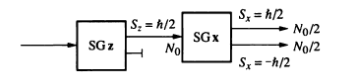
\includegraphics[width=0.6\textwidth]{2SGs.png}
    \caption{Esquema da situação descrita no enunciado. Figura retirada de \cite{townsend}.}
    \label{fig:2sg}
  \end{figure}
    
  \item Qual é a fração de partículas que deixa o segundo SG em relação ao que deixa o primeiro SG? Justifique a resposta.

  \textbf{Resolução:}
  
  Suponha, como na figura, que $N_0$ partículas saem do primeiro SG$_z$. Como a componente inferior está bloqueada, todas estas partículas estão no estado $\ket{+}_z$, o autoestado de $S_z$ com autovalor $\hbar/2$.
  O segundo SG mede a componente do momento angular na direção x. Como uma medida de $S_x$ para uma partícula no estado $\ket{\psi}$ fornece $+\hbar/2$ com probabilidade $\left|\prescript{}{x}{\left\langle +|\psi\right\rangle}\right|^2$, a probabilidade de uma partícula no estado $\ket{+}_z$ sair de SG$_x$, que possui a saída inferior bloqueada, é 
  \[
  p = \left|\prescript{}{x}{\left\langle +|+\right\rangle}_{z}\right|^2 
  \]

  Nos dados da prova, foi fornecido que os autovetores do operador spin na direção $\hat{n} = \sin \theta \cos \phi \hat{x} + \sin \theta \sin \phi \hat{y} + \cos \theta \hat{z}$ na base comum de $S^2$ e $S_z$ são

\[
  \ket{S_n = +\frac{\hbar}{2}} = \begin{pmatrix} \cos(\theta/2) \\ \sin(\theta/2)e^{i\phi} \end{pmatrix}
\]
\[
  \ket{S_n = -\frac{\hbar}{2}} = \begin{pmatrix} \sin(\theta/2) \\ -\cos(\theta/2)e^{i\phi} \end{pmatrix}
\]
  Para $\hat{n} = \hat{x}$ temos $\theta = \pi/2$ e $\phi = 0$, portanto
  \[
    \ket{+}_x = \begin{pmatrix} \frac{1}{\sqrt{2}} \\ \frac{1}{\sqrt{2}} \end{pmatrix}
  \]
  Podemos agora calcular a probabilidade pedida; Como
  
  \begin{align*}
  \prescript{}{x}{\left\langle +|+\right\rangle}_{z} &= \begin{pmatrix} \frac{1}{\sqrt{2}} & \frac{1}{\sqrt{2}} \end{pmatrix}
  \begin{pmatrix}
  1 \\ 0
  \end{pmatrix} \\
  &= \frac{1}{\sqrt{2}}
  \end{align*}
  
  \noindent temos $p = 1/2$. Em média, se saem $N_0$ partículas de $SG_z$, sairão $N_0/2$ partículas de $SG_x$.
  
  \item Se adicionarmos um terceiro SG, após os dois primeiros SG, que transmite somente a componente superior de $S_z$, qual fração de partículas que deixa o terceiro SG em relação ao que deixa o primeiro SG? Justifique a resposta.
  
  \textbf{Resolução:}
  
  \begin{figure}[H]
    \centering
    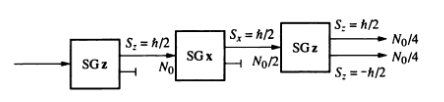
\includegraphics[width=0.6\textwidth]{3SGs_com_bloqueio.png}
    \caption{Esquema da nova situação. Figura retirada de \cite{townsend}.}
    \label{fig:3sg}
  \end{figure}
  
  Agora temos a situação descrita na Figura \ref{fig:3sg}. Note que as partículas que entram no último SG$_z$ estão no estado $\ket{+}_x$. A probabilidade de emergirem é então
  
  \begin{align*}
  p &= \left|\prescript{}{z}{\left\langle +|+\right\rangle}_x\right|^2 \\
  &= 1/2
  \end{align*}
  
  Se entram $\frac{N_0}{2}$ partículas, sairão $\frac{N_0}{4}$ partículas, portanto.
  
  \item Agora o segundo SG com o campo na direção x, ambos os feixes, o superior e o inferior e o terceiro SG na direção z transmite apenas na direção inferior. Qual a fração de partículas que deixa o terceiro SG em relação ao que deixa o primeiro SG? Justifique a resposta.
  
  \textbf{Resolução:}
  Após passar pelo segundo SG, todas as partículas colapsam no estado $\ket{+}_x$ ou $\ket{-}_x$: o feixe entrando o último SG é portanto uma mistura de $N_0$ partículas nestes dois estados: $\frac{N_0}{2}$ no estado $\ket{+}_x$ e $\frac{N_0}{2}$ no estado $\ket{-}_x$. Como \textbf{ambas} as partículas possuem probabilidade $1/2$ de sair na direção inferior, pois
  
  \[
  \left|\prescript{}{z}{\left\langle -|+\right\rangle}_x\right|^2 = \left|\prescript{}{z}{\left\langle -|-\right\rangle}_x\right|^2
  \]
  
  \noindent o número de partículas saindo na parte inferior do terceiro SG será
  
  \[
  \left(\frac{N_0}{2} + \frac{N_0}{2}\right) \frac{1}{2} = \frac{N_0}{2}
  \]
  
  \textit{Observação:} Note que o resultado deste último item depende que a medição realizada por $S_x$ de fato colapse os estados da partícula dos autoestados de $S_x$ antes de misturarmos as partículas de novo. Ou seja, devemos ser capazes de determinar se as partículas do feixe entrando o último SG$_z$ sairam na saída superior ou inferior de SG$_x$. É possível construir um aparato de Stern-Gerlach modificado, descrito por Feynman e discutido em \cite{townsend}, onde orientamos três magnetos de forma que partículas de spin up e down seguem trajetórias diferentes dentro do aparelho (ou pelo menos seguiriam classicamente - lembre-se que o conceito de trajetória não está bem definido em mecânica quântica), se juntando na saída (cf. Figura \ref{fig:sg_modificado}).
  
  \begin{figure}[H]
    \centering
    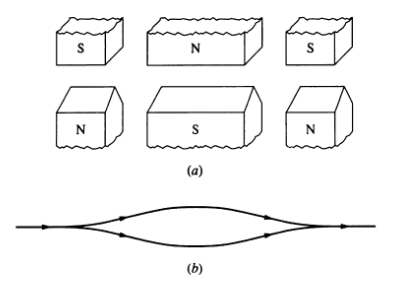
\includegraphics[width=0.6\textwidth]{modified_SG.png}
    \caption{Aparato de Stern-Gerlach modificado. Figura retirada de \cite{townsend}.}
    \label{fig:sg_modificado}
  \end{figure}
  
  A diferença aqui é que sem interromper a trajetória superior ou inferior, não conseguimos saber qual das duas trajetórias a partícula seguiu: na verdade, esta pergunta sequer faz muito sentido. O estado da partícula, portanto, não colapsa em um dos autoestados do momento angular na direção selecionada pelo aparato SG, se mantendo inalterado. Se trocássemos o segundo aparato SG (SG$_x$) neste exercício por um destes aparatos modificados, o feixe de $N_0$ partículas emergindo dele estaria no mesmo estado em que entrou, $\ket{+}_z$. Neste caso, portanto, \textbf{nenhuma partícula emergiria do último SG$_z$ na saída de baixo}!
  Uma discussão interessante destes aspectos do experimento de Stern-Gerlach pode ser lida na seção 1.2 do livro de Townsend (\cite[1]), disponível nas melhores livrarias digitais russas.
\end{enumerate}

%FIM DOS PROBLEMAS
\end{enumerate}
\end{document}

\printbibliography
